\documentclass{article}
\usepackage[utf8]{inputenc}
\usepackage[top=1in]{geometry}
\usepackage{graphicx}
\usepackage{booktabs}
\usepackage{tikz}
\usetikzlibrary{circuits.logic.US,positioning,calc} 
\input{sym}
\title{Homework 2}
\author{Max marks: 105}
\date{Due on September 18, 2023, before class. Please submit both in brightspace
  and in person in paper this time. Grading on paper is easier.}
\newtheorem{prob}{Problem}

\newcommand{\bx}{\bar{x}}
\newcommand{\by}{\bar{y}}
\newcommand{\bz}{\bar{z}}
\begin{document}

\maketitle

\begin{figure}
\begin{minipage}{0.5\linewidth}
\centering
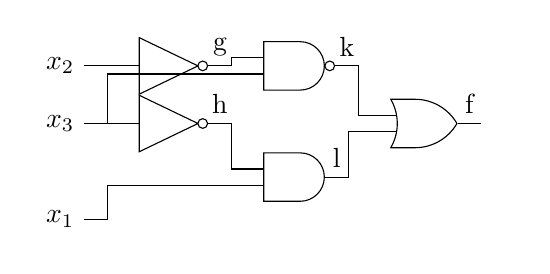
\begin{tikzpicture}[circuit logic US]
  \matrix[column sep=7mm]{
    \node (x2) {$x_2$}; & \node [not gate] (nx2) {};&  \node [nand gate] (x1nx2) {}; & \\
    \node (x3) {$x_3$}; & \node [not gate] (nx3) {};&  & \node [or gate] (f) {};\\
    & & \node [and gate] (x1nx3) {}; &  & \\
    \node (x1) {$x_1$}; & &  & \\
  };
  \draw (x2.east) -- ++(right:3mm) |- (nx2.input);
  \draw (nx2.output) to [edge label=g] ++(right:3mm) |- (x1nx2.input 1);

  \draw (x3.east) -- ++(right:3mm) |- (x1nx2.input 2);
  \draw (x3.east) -- ++(right:3mm) |- (nx3.input);
  \draw (nx3.output) to [edge label=h] ++(right:3mm) |- (x1nx3.input 1);

  \draw (x1.east) -- ++(right:3mm) |- (x1nx3.input 2);

  \draw (x1nx2.output) to [edge label=k] ++(right:3mm) |- (f.input 1);
  \draw (x1nx3.output) to [edge label=l] ++(right:3mm) |- (f.input 2);

  \draw (f.output) to [edge label=f] ++(right:3mm);

\end{tikzpicture}
\caption{A three-input circuit}
\label{fig:fig-2.24a}
\end{minipage}
\begin{minipage}{0.5\linewidth}
    \centering
    \begin{tabular}{ccc|c}
      \toprule
      $x_1$ & $x_2$ & $x_3$ & $f(x_1, x_2, x_3)$ \\
      \midrule
      0 & 0 & 0 & 0 \\
      0 & 0 & 1 & 1 \\
      0 & 1 & 0 & 1 \\
      0 & 1 & 1 & 0 \\
      1 & 0 & 0 & 1 \\
      1 & 0 & 1 & 1 \\
      1 & 1 & 0 & 1 \\
      1 & 1 & 1 & 0 \\
      \bottomrule
      \end{tabular}
    \caption{A three-variable function}
    \label{fig:fig-2.23}
\end{minipage}
\end{figure}

\begin{prob}
  Consider the circuit in Figure~\ref{fig:fig-2.24a}. Write the circuit as:
  \begin{enumerate}
    \item Boolean expression [5 marks]
    \item Truth table [10 marks]
    \item Venn diagram. [5 marks]
  \end{enumerate} (Total 20 marks)
\end{prob}

\begin{prob}
Represent the function in Figure~\ref{fig:fig-2.23} in the form of a 
\begin{enumerate}
  \item Venn diagram [5 marks]
  \item Boolean expression [5 marks]
  \item ANSI symbol network [5 marks]
  \item Timing diagram [5 marks]
\end{enumerate}
    Also, find its minimal sum-of-products form [5 marks].
    (Total 25 marks).
\end{prob}

\begin{prob}
Use algebraic manipulation to simplify the function $f = x_1x_3 + x_1x_2 + \bx_1 \bx_2 x_3 + \bx_1 \bx_2 \bx_3$. If the function is already in its simplest form, say so. [10 marks]
\end{prob}

\begin{prob}
Use algebraic manipulation to simplify the function $f = x_1 x_2\bx_3 + x_1\bx_2x_4 + x_1\bx_2 x_3\bx_4$. If the function is already in its simplest form, say so. [10 marks]
\end{prob}

\begin{prob}
Use algebraic manipulation to prove that $(x+y)\cdot(x+\bar{y}) = x$. [10 marks].
\end{prob}

\begin{prob}
Determine whether or not the following expressions are valid, i.e., whether the
left- and right-hand sides represent the same function.
[10 marks]
\begin{enumerate}
    \item $x_1 \bx_3 + x_2 x_3 + \bx_2 \bx_3 = (\bx_1 + \bx_2 + x_3)(x_1 + x_2 + \bx_3)(\bx_1 + x_2 + \bx_3)$
    \item $(x_1 + x_3)(\bx_1 + \bx_2 + \bx_3)(\bx_1 + x_2) = (x_1 + x_2)(x_2 + x_3)(\bx_1 + \bx_3)$
\end{enumerate}
\end{prob}

\begin{prob}
Design the simplest sum-of-products circuit that implements the function $f (x_1
, x_2 , x_3, x_4 ) = \sum m(3, 4, 6, 7, 8)$.[10 marks]
\end{prob}

\begin{prob}
Design the simplest product-of-sums circuit that implements the function $f (x_1 , x_2 , x_3 ) = \prod M (0, 2, 5, 6)$.[10 marks]
\end{prob}


%\bibliography{main}
%\bibliographystyle{plain}
\end{document}
